\documentclass[a4paper,11pt, twocolumn]{article}
\usepackage[margin=0.8in]{geometry}
\usepackage{xcolor}
\usepackage{graphicx} %package to manage images
\graphicspath{ {./images/} }

\title{1.3.3 Networks}
\author{Revision sheet}
\date{}

\usepackage{fancyhdr}
\pagestyle{fancy}
\fancyhead{} % clear all header fields
\renewcommand{\headrulewidth}{0pt} % no line in header area
\fancyfoot{} % clear all footer fields
\renewcommand{\footrulewidth}{0.4pt}
\fancyfoot[C]{\thepage} % page number in centre of the page
\fancyfoot[R]{\footnotesize Thomas Boxall \\ Images from Physics \& Maths Tutor} % right hand footer has author name on top line and images reference on bottom line
\fancyfoot[L]{\footnotesize 1.3.3 Networks \\ Revision sheet} % left hand footer has title of document on top line and 'Revision Sheet' on bottom line


\begin{document}

\maketitle
\thispagestyle{fancy}

% CONTENTS OF THE REVISION SHEET HERE

\section{Structure of the Internet}
\subsection{Physical Structure of the internet}
The internet is comprised of a number of nodes and cables or wireless connections which connect them. To connect different continents together, there are a number of backbone trans-continental cables which are run along the sea bed. National ISPs (internet service providers) connect to these then distribute the data to individual homes and businesses.
\subsection{URLs}
Uniform Resource Locators are the full addresses of an internet resource. They specifiy the location of a single resource on the internet. A typical URL might contain the resource name and file type so the browser knows what to request from the web server. An example is shown below:\\
\verb|https://www.domainname.com/folder/|\\ \verb|subfolder/webpage.html#element|

\subsection{Domain Name System}
\subsubsection{Internet Registrars}
Internet registrars hold records of all existing website names and details of domains which are available to purchase. Internet registries are five global organisations governed by the Internet Corporation for Assigned Names and Numbers (ICANN) with worldwide databases that hold the domain names which are currently in use; the information of the individual/company who registered them and the IP address of the web server which the website is hosted on. 
\subsubsection{Domain Names}
A domain name identifies the area that the internet resource comes from. These are structured into a hierarchy of smaller domains and are written as a string represented by full stops. Countries have their own Top Level Domains, EG.\verb|.uk|.  
Each domain name has at lease one IP address. The DNS (Domain Name Server) catalogues all the domain names and IP addresses into global directories which DNS can access in order to find the IP address for a resource. When a user enters a URL for a website, the browser retrieves the corresponding IP address from a local DNS server then the IP address is used to retrieve the content requested. We use URLs rather than IP addresses directly, as they are easier to remember. 
\subsection{Fully Qualified Domain Name}
A FQDN is one that includes the server name. For example, \verb|www.| or \verb|mail.|
\subsection{IP Addresses}
An Internet Protocol Address (IP Address) is uniquely assigned to all network devices. It indicates where a packet of data is being sent or where it has been sent from. Routers can use this address to direct packets accordingly.
\subsection{Wide Area Networks}
WANs are generally spread out over a large geographical area, sometimes across continents. For example, the NHSs network would be defined as a WAN. WANs generally rely on third party carriers or connections such as those provided by BT.
\subsection{Local Area Networks}
LANs consist of a number of computing devices on a single site or in a single building; so in a small geographical area.
\subsection{Topologies}
There are a number of topologies \textit{(diagrams which show the physical or logical layout of a network)} which are fundamental to networking.
\subsubsection{Physical Bus Topology}
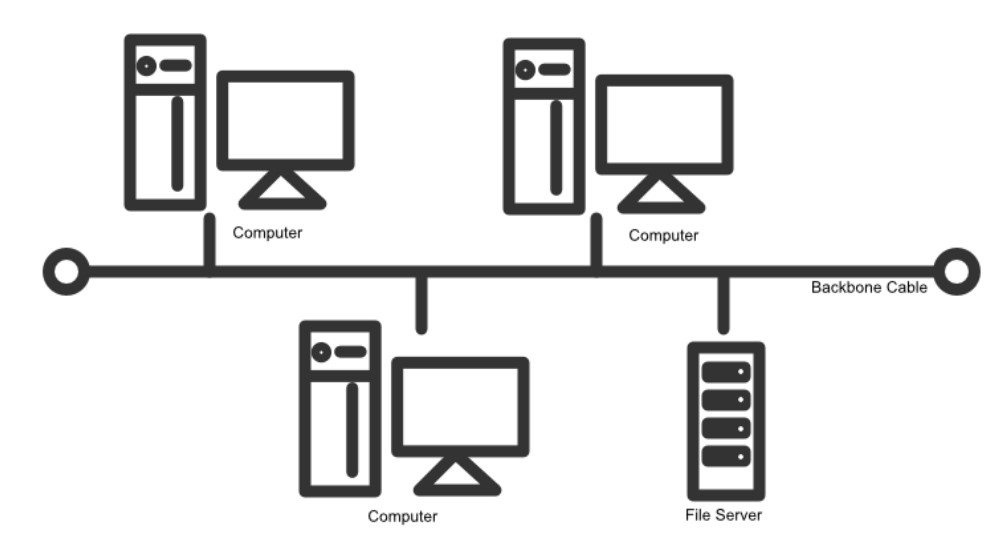
\includegraphics[width=0.45\textwidth]{topoBus.jpg}\\
In this topology, all computers are connected to a single cable. The ends of the cable are connected to a terminator. Advantages: inexpensive to install and doesn't require any additional hardware. Disadvantages: If the backbone fails, the network data can no longer be transmitted to any of the nodes; performance degrades with heavy traffic; low security (all the computers on the network can see all data transmissions).
\subsubsection{Physical Star Topology}
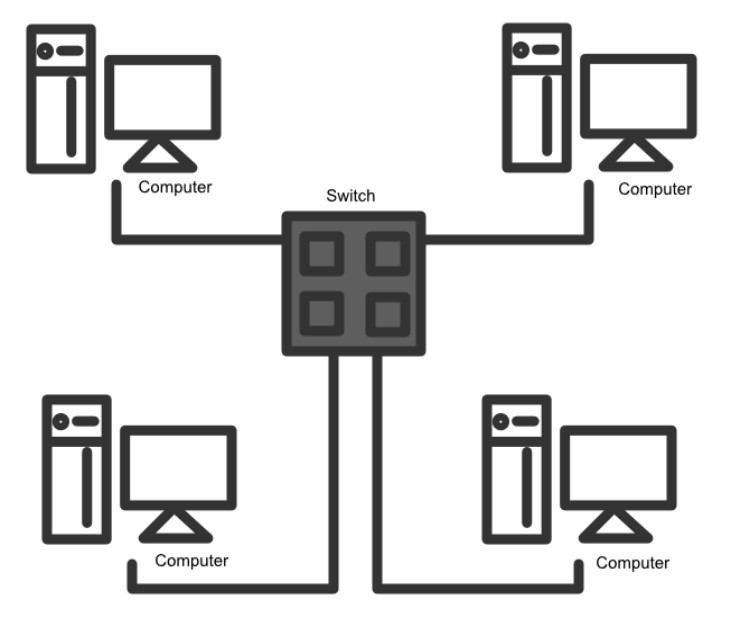
\includegraphics[width=0.45\textwidth]{topoStar.jpg}\\
Star topologies have a central node which is usually a switch or router, whose purpose is to transmit messages. The switch keeps a record of the unique MAC addresses of each device on the network and can identify which particular node needs the data transmitted to it.
Advantages: Simple to isolate and fix faults; Consistent performance even with heavey use; Each node has a direct connection to the server; Can add new nodes to the network without disrupting other nodes. Disadvantages: Needs lots of cable to install - can be expensive; if central device fails, data can no longer be transmitted to any of the nodes.
\subsubsection{Physical Mesh Topology}
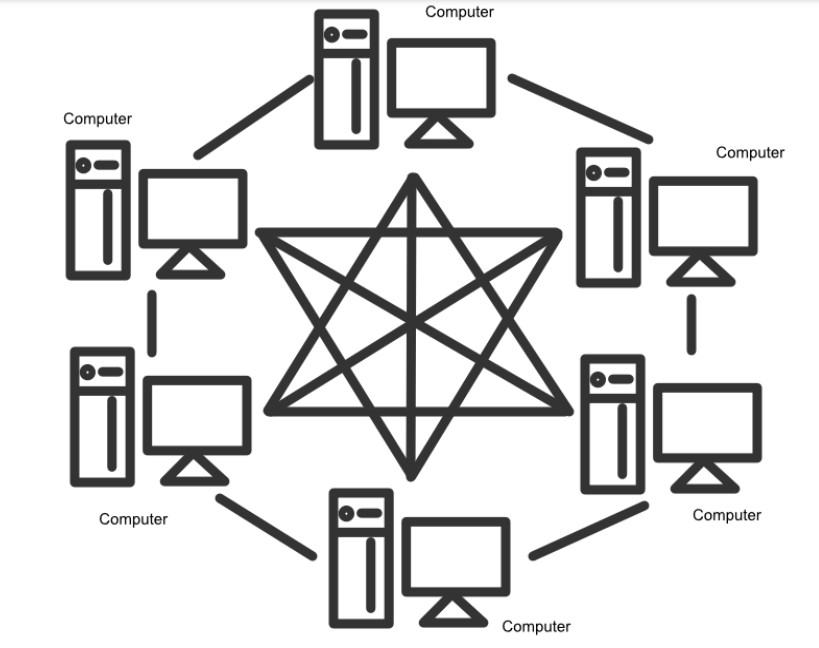
\includegraphics[width=0.45\textwidth]{topoMesh.jpg}\\
Mesh topologies have every node connected to every other node. They are most commonly found with wireless technology. Advantages: No cabling costs; extra nodes are automatically incorporated; nodes don't go through a central switch, improves speed. Disadvantages: Maintaining the network is difficult; If using wired connections - a massive amount of wire is required; If using wireless connections - all devices need to have suitable wireless connectivity, this can increase cost.
\subsubsection{Client-Server}
Client-server networks consist of clients (terminals) connected to a single server. The server is a powerful central computer which holds all of the important information and resources, it has greater processing power than the terminals. Clients can request to use the server. Advantages: more secure as data is stored in one location; central backups are carried out so no need for individual backups; data and resources can be shared between clients. Disadvantages: Expensive to setup; Specialist staff required to maintain the server; Functionality of the terminals depends on the server, if this fails, performance fails.
\subsubsection{Peer-to-Peer}
This is a network in which computers are connected to each other so that they can share files. Each device effectively acts as both a server and client, so it can provide and request resources. P2P networks are used in piracy as it is almost impossible to trace the origin of files. Advantages: Cheaper to setup, allows users to share resources; easy to maintain; not dependent on a central server; specialist staff not required. Disadvantages: impossible to trace the origin of files; backups must be performed of each computer separately; poorer security; may be difficult to locate resources.
\subsection{Wireless connections}
\subsubsection{Wi-Fi}
Wi-Fi is a local area wireless technology that enables you to connect a device to a computer network or to the internet via a wireless connection. It has a standard connection standard which makes use of protocols.
\subsubsection{Wireless Access Point}
In order to connect to a wireless network, a computer device needs a wireless network adapter. To connect to the internet, the WAP usually connects to a router but could be an inbuilt part of the router itself.

\section{Internet Communications}
\subsection{Packets}
Data that is to be transported across the internet is broken down into a series of packets. The size of each packet is generally between 500 and 1500 bytes. Each packet contains a header and payload, some also use a trailer section which contains a checksum. The header contains the sender and recipients IP addresses, the protocol being used, the packets number in sequence (eg, packet 1 of 12) and the Time To Live (TTL) which tells routers how long to let the packet bounce around for before being discarded. The payload contains the data which is being transmitted. The trailer section's checksum is used to ensure that the packet has arrived safely at its destination, there are a variety of ways in which this can be done.
\subsection{Switching}
There are a number of different ways in which data can be sent across a network.
\subsubsection{Circuit Switching}
This is where the route which the data will take is setup prior to the message being sent as a complete block. There is no delay at the destination as the message is complete on arrival. This works much the same as a phone call.
\subsubsection{Packet Switching}
Data is split into packets which are inspected at each node on the network and redirected until they reach their destination. It doesn't require the route to be determined before the packets set off and the packets have to be reassembled at the destination. The packets will generally take different routes so might arrive in the wrong order. 
\subsection{Routers}
Routers are used to connect at least two networks, commonly two LANs or WANs, or to connect a LAN to its ISP network. Travelling from one router to another router is called a hop. A routers purpose is to read the recipients IP address in the header of each packet and forward it onto the recipient via the fastest and least congested route. Routers use routing tables to store the details of other network devices and the most efficient routes to them. A routing algorithm (similar to shortest path algorithm like Dijkstra's Algorithm) is used to find the best routes to send packets down.
\subsection{Gateways}
Gateways are used between networks to translate different protocols. All of the header data is stripped from the packet leaving only the raw data and the new header is added, complying with the new protocol. Gateways then act like routers and send the packets on their way again.
\subsection{Media Access Control Addresses}
Every computer device which is capable of being part of a network must have a wired or wireless Network Interface Card (NIC). Each NIC has a unique MAC address which is assigned and hard-coded into the card by the manufacturer. MAC addresses uniquely identify the device, they are 48 bits long and are written as 12 HEX digits.

\section{The Importance Of Protocols and Standards}
A protocol is a set of rules defining how two computers communicate with each other. Protocols are standard across all devices, meaning all devices should be able to communicate, regardless of manufacturer.
\subsection{The TCP/IP Protocol Stack}
The \textit{Transmission Control Protocol / Internet Protocol} protocol stack is a set of networking protocols that work together as four interconnected layers, passing outgoing data down the stack and incoming data up the stack during network communication.
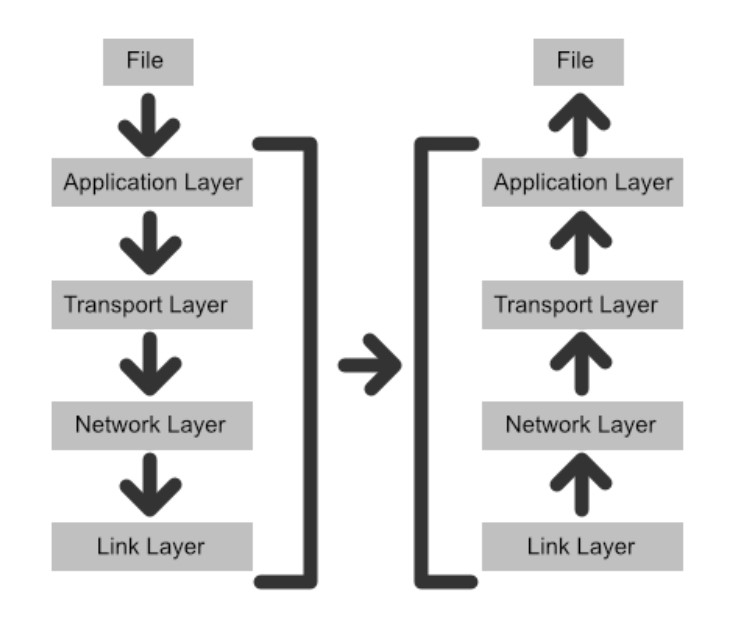
\includegraphics[width=0.45\textwidth]{tcpIP.jpg}\\
Various protocols are used in each layer, each with different roles. At each layer, the data is encapsulated in an envelope containing new packet data. On the receiving end, as the packet moves up the stack, the data is unwrapped, revealing the data on its own. 
\subsubsection{The Application Layer}
The application layer uses protocols relating to the application being used to transmit data over a network, usually the internet. For example, if the application is a browser, it would select an appropriate higher-level communication such as HTTP, POP3 or FTP.
\subsubsection{The Transport Layer}
The transport layer uses the Transmission Control Protocol to establish an end-to-end connection with the recipient computer. The data is then split into packets, and labelled with the packet number in sequence and port number (eg, Packet 1 of 12; Port 80).
\subsubsection{The Internet (Network) Layer}
The internet layer adds the source and destination IP address. Routers operate on the internet layer and will use these IP addresses in their work.
\subsubsection{The Link Layer}
The link layer is the physical connection between network nodes and it adds the MAC addresses of the source and destination computers. If the destination isn't on the same network as the source, the MAC address of the first router is set to the destination MAC address, this is the corrected at the first router.
\subsection{Other useful protocols}
There are a number of other useful protocols.
\subsubsection{FTP}
File Transfer Protocol (FTP) is used to transfer files over networks. There are some GUI applications which can be used, as well as command line applications.
\subsubsection{POP3, IMAP, SMTP}
Post Office Protocol V3 is responsible for retrieving emails from a mail server that temporarily stores incoming mail. When they are transferred off of the mail server, they are deleted from the server. Internet Message Access Protocol is another email protocol designed to keep emails on the server. Simple Mail Transfer Protocol is used to transfer outgoing emails from one server to another or from an email client to the server when sending an email. 
\subsection{Physical and Logical}
There are two key different types of protocols, Physical and Logical protocols. These link to the TCP/IP stack.
\subsubsection{Physical Protocols}
This relates to the hardware used for the transmission. It uses the lower layers of the TCP/IP stack.
\subsubsection{Logical Protocols}
This relates to the software used for the transmission. It uses the upper layers of the TCP/IP stack.

\section{Network and Security Threats}
\subsection{Firewalls}
A firewall is designed to prevent unauthorised access to a network. It generally consists of a separate computer containing two NICs, with one connected to the internal network and the other connected to the external network. Using special firewall software, each data packet that attempts to pass between the two NICs is analysed against the packet filter (preconfigured rules) then accepted or rejected. A firewall may also act like a proxy server. 
\subsection{Packet Filtering}
Packet Filtering, controls network access according to the network administrators rules and policies by examining the source and destination IP addresses in packet headers. If the IP addresses match those recorded on the admin's permit list then they are accepted. Static filtering can also block packets based on the protocols being used and the port numbers they are trying to access. For example, Telnet (remote access software) uses port 23, any request using port 23 might be dropped or rejected based on the network admin's rules. Dropped packets are quietly removed whereas rejected packets will cause a rejection notice to be sent back to the user.
\subsection{Proxy Servers}
A proxy server intercepts all packets entering and leaving a network, hiding the true network addresses of the source from the recipient. This enables privacy and anonymous surfing. Proxy servers also cache frequently visited websites, this speeds up access to the site and reduces web traffic. A proxy server might serve thousands of users. Some proxy servers for example, the ones at a school, will filter the content in accordance with the acceptable usage policy and may keep a log of which user requested the data.
\subsection{Worms, Trojans and Viruses}
These are all types of malware. They are all designed to cause inconvenience, loss or damage to programs, data or computer systems.
\subsubsection{Virus and Worm subclass}
These have the ability to self-replicate by spreading copies of themselves.
\subsubsection{Trojans}
These will commonly open 'back doors' to devices that the creator of the trojan can exploit. Trojans cannot self replicate.
\subsection{System vulnerabilities}
Malware exploits vulnerabilities in our systems, which may have come from human error or software bugs. People are often the weakest point in security. Passwords are no guarantee of protection against unauthorised access since these are not always treated with the correct level of security.
\subsection{Protection against Threats}
Code quality is a primary vulnerability of systems. Regular operating system and antivirus software updates ill also help to reduce the risk of attack. Virus checkers usually scan for all other malware types, not just viruses. 
\end{document}